% !TEX root = ./document.tex

\documentclass{article}
\usepackage{mystyle}
\usepackage{myvars}
\usepackage{graphicx}
\graphicspath{{./figs/}}
\usepackage{wrapfig}


%-----------------------------

\begin{document}

	\maketitle % Insert title

	\thispagestyle{fancy} % All pages have headers and footers


%-----------------------------
%	ABSTRACT
%-----------------------------

	\begin{abstract}
		\noindent [TODO ].
	\end{abstract}

%-----------------------------
%	TEXT
%-----------------------------


	\section{Introduction}
	\label{sec:intro}

			\paragraph{}
			[TODO ]


	\section{Supervised Learning}
	\label{sec:supervised-learning}

		\paragraph{}
		[TODO ]

		\paragraph{Error Measures}
		\label{paragraph:error-measures}
		[TODO ]

		\begin{itemize}
			\item [TODO ]
		\end{itemize}

		\paragraph{Experimental Strategies}
		\label{paragraph:experimental-strategies}
  	[TODO ]

		\begin{itemize}
			\item
				\textbf{Holdout}:
				[TODO ]

			\item
				\textbf{Repeated Holdout}:
				[TODO ]

			\item
				\textbf{Cross Validation}:
				[TODO ]

			\item
				\textbf{Repeated Cross Validation}:
				[TODO ]

		\end{itemize}

		\subsection{Decision Trees}
		\label{sec:decision-trees}

			\paragraph{}
			[TODO ]

		\subsection{Rule Based Systems}
		\label{sec:decision-trees}

			\paragraph{}
			[TODO ]

		\subsection{Instance Based Learning}
		\label{sec:decision-trees}

			\paragraph{}
			[TODO ]

		\subsection{Bayes Learning}
		\label{sec:decision-trees}

			\paragraph{}
			[TODO ]

		\subsection{Linear Classifiers}
		\label{sec:decision-trees}

			\paragraph{}
			[TODO ]

		\subsection{Neural Networks}
		\label{sec:decision-trees}
		
			\subsubsection{Perceptron model}
			
			\begin{figure}[htpb!]
				\centering
				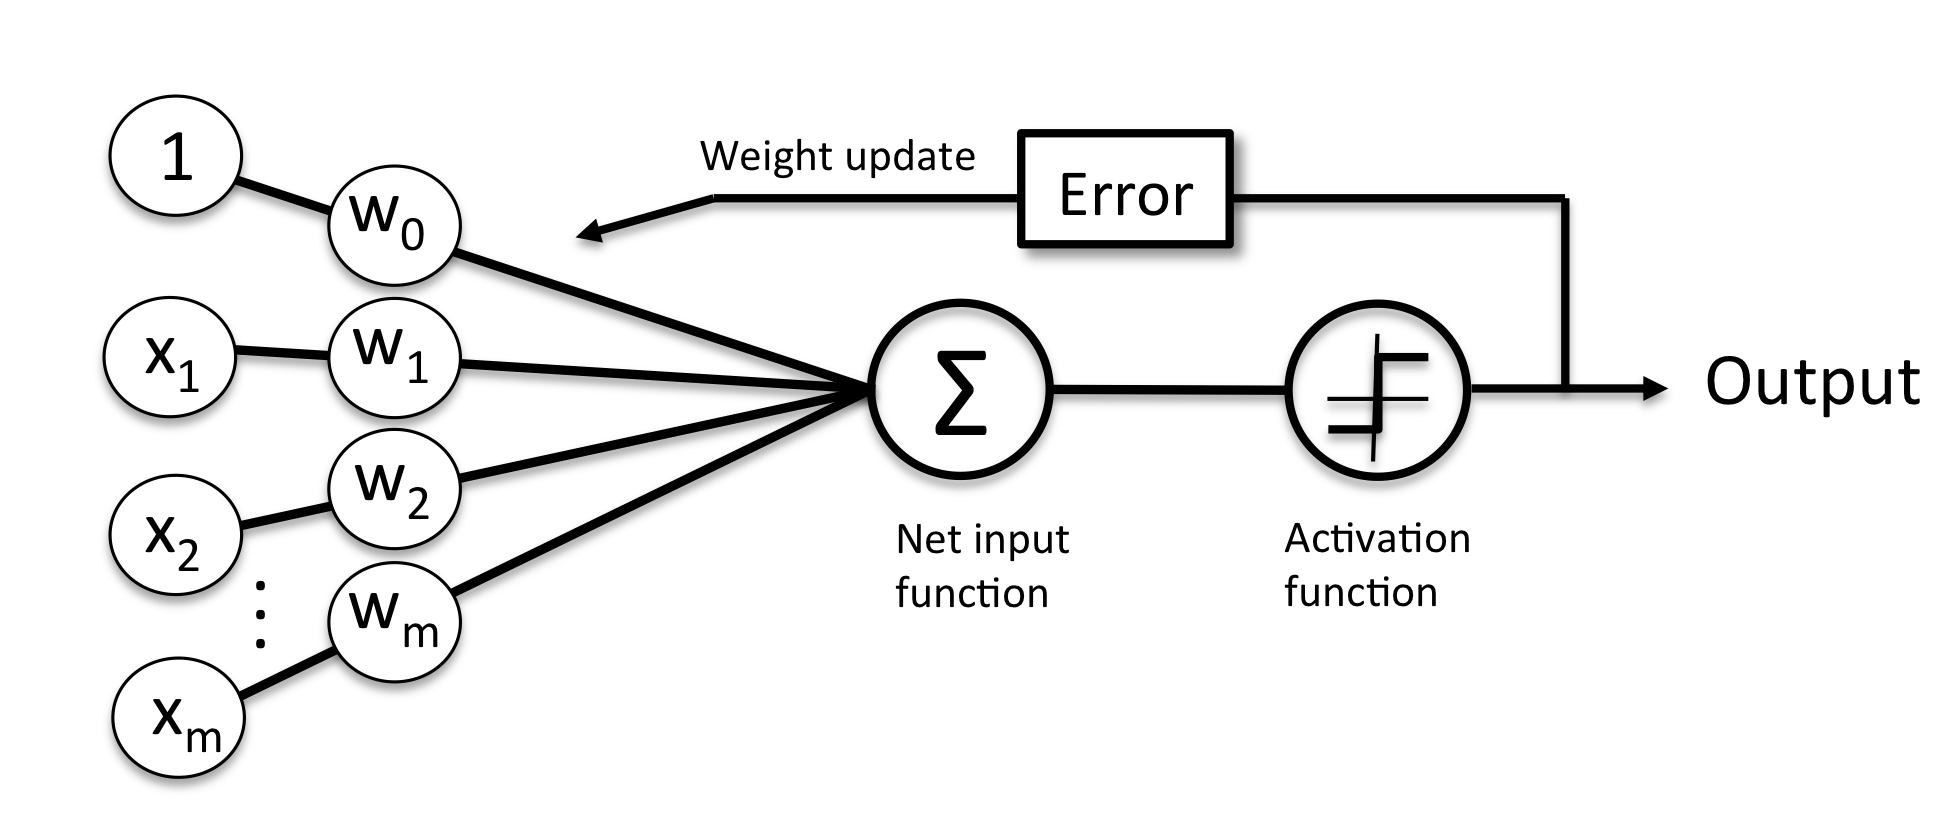
\includegraphics[scale=.1]{perceptron-concept}
				\caption{General concept of perceptron}
				\label{fig:perceptron-concept}
			\end{figure}
			
			\paragraph{Perceptron's structures}
			\begin{equation*}
				w = \begin{bmatrix}
						w_1 \\
						\vdots \\
						w_m
					\end{bmatrix}, x = 
					\begin{bmatrix}
						x_1 \\
						\vdots \\
						x_m
					\end{bmatrix}
			\end{equation*}

			\paragraph{Ouput equation}			
			\begin{equation*}
				z = w_1 x_1 + \dots + w_m x_m = \boldsymbol{w^T x}
			\end{equation*}
			
			
			\paragraph{Activation function}
			
			\begin{wrapfigure}{o}{.5\textwidth}
				\centering
				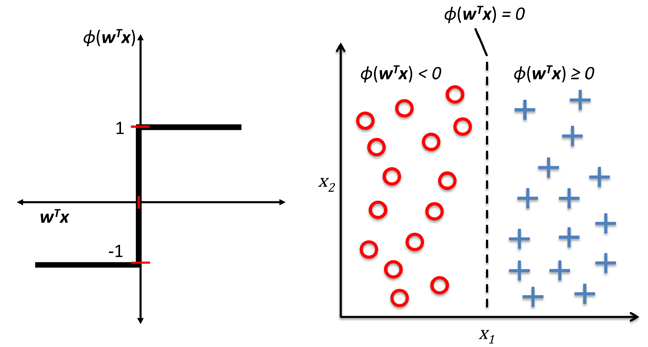
\includegraphics[scale=.25]{activation-function}
				\caption{Activation function}
				\label{fig:activation-function}
			\end{wrapfigure}
			
			\begin{equation*}
				\phi(z) = \begin{cases}
					1 &\mbox{if } z \geq \theta \\
					-1 &\mbox{otherwise}
				\end{cases}
			\end{equation*}
			
			\paragraph{Update of weight vector}
			
			\begin{equation*}
				\begin{aligned}
					w_j &:= w_j + \Delta w_j \\
					\Delta w_j &= \eta(y^{(i)} - \hat{y}^{(i)}) x^{(i)}_j
				\end{aligned}
			\end{equation*}

			\subsubsection{Adaptive linear neurons (ADALINE)}
			
			\begin{figure}[htpb!]
				\centering
				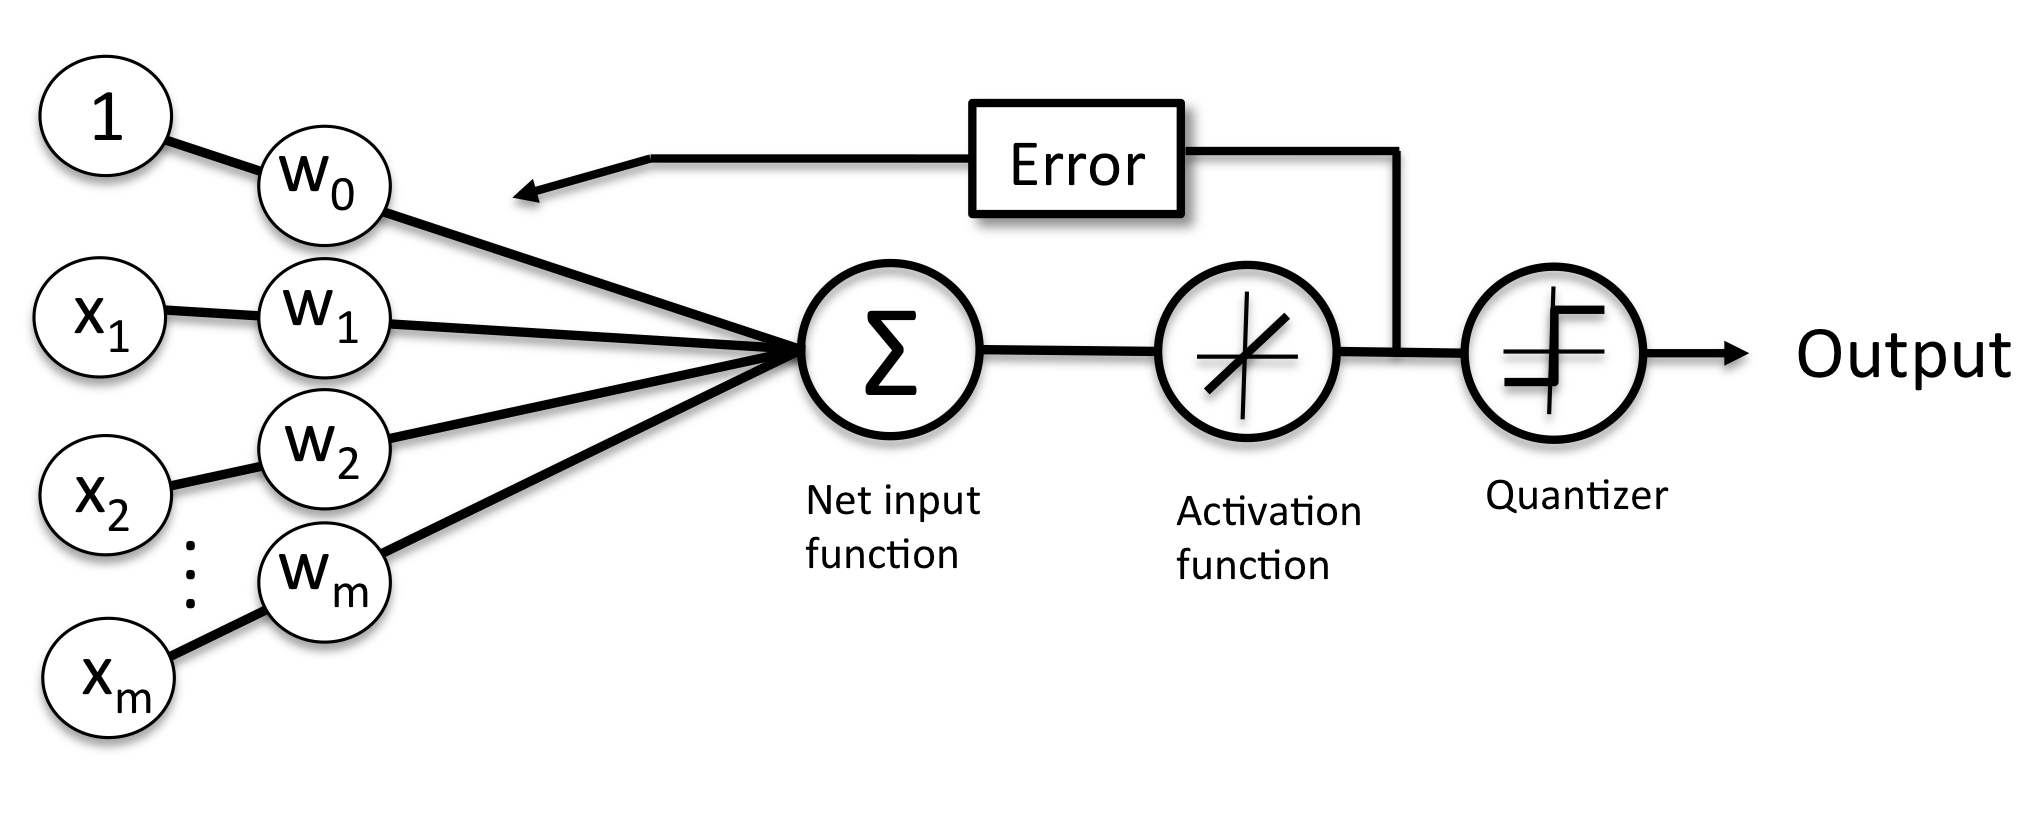
\includegraphics[scale=.1]{adaline-concept}
				\caption{General concept of adaline perceptron}
				\label{fig:adaline-concept}
			\end{figure}
			
			\paragraph{Cost function}
			
			\begin{wrapfigure}{o}{.5\textwidth}
				\centering
				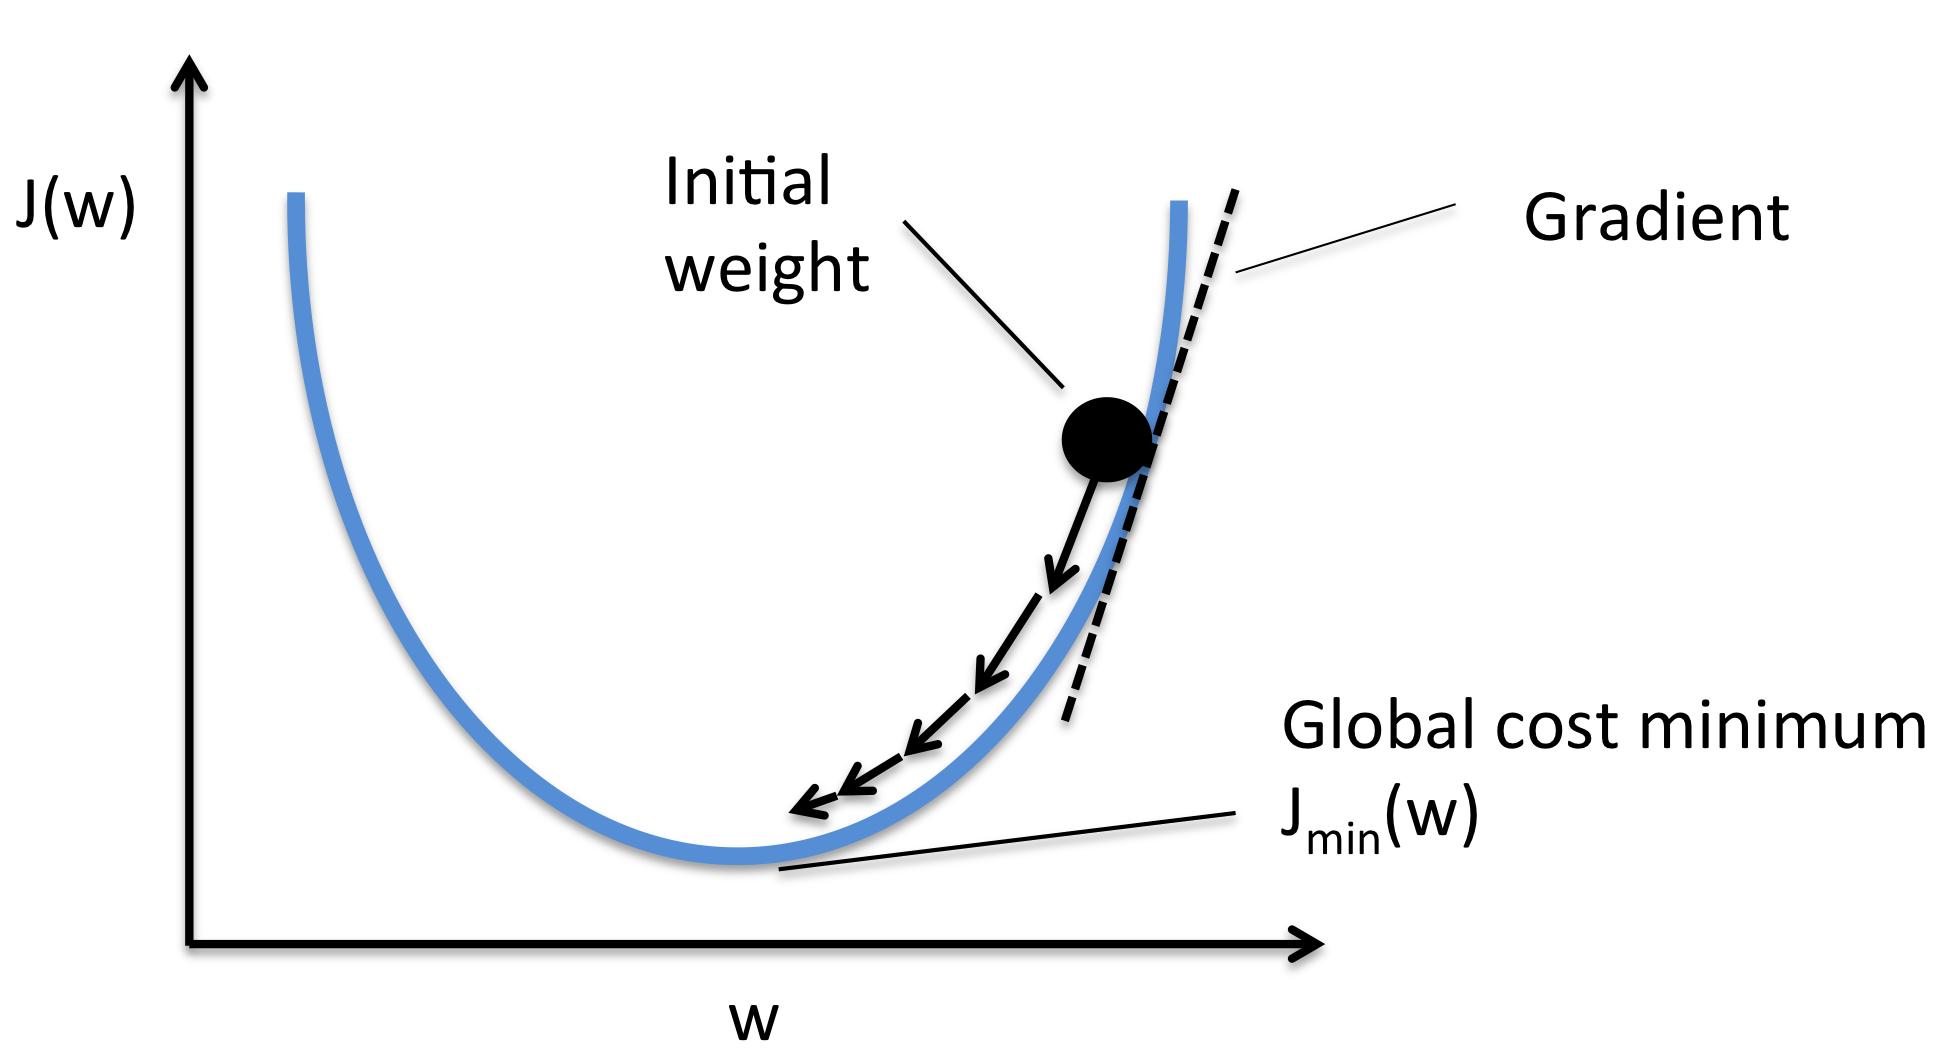
\includegraphics[scale=.1]{gradient-descend}
				\caption{Gradient descent}
				\label{fig:gradient-descend}
			\end{wrapfigure}
						
			\begin{equation*}
				J(w) = \frac{1}{2} \sum_i (y^{(i)}-\phi(z^{(i)}))^2
			\end{equation*}
			
			\paragraph{Update of weight vector}
			
			\begin{equation*}
				\begin{aligned}
					w_j &:= w_j + \Delta w_j \\
					\Delta w_j &= -\eta\nabla J(w) = \eta\sum_i (y^{(i)} -\phi(z^{(i)}))x^{(i)}_j
				\end{aligned}
			\end{equation*}
			
			\paragraph{Features standarization}
			
			\begin{equation*}
				x'_j = \frac{x_j - \mu_j}{\sigma_j}
			\end{equation*}
			
			\vspace{2cm}
			

	\section{Unsupervised Learning}
	\label{sec:unsupervised-learning}

			\paragraph{}
			[TODO ]

%-----------------------------
%	Bibliographic references
%-----------------------------

	\nocite{subject:taa}
	\nocite{packt:py-machine-learning}

  \bibliographystyle{alpha}
  \bibliography{bib}

\end{document}
